% Template for PLoS
% Version 3.1 February 2015
%
% To compile to pdf, run:
% latex plos.template
% bibtex plos.template
% latex plos.template
% latex plos.template
% dvipdf plos.template
%
% % % % % % % % % % % % % % % % % % % % % %
%
% -- IMPORTANT NOTE
%
% This template contains comments intended 
% to minimize problems and delays during our production 
% process. Please follow the template instructions
% whenever possible.
%
% % % % % % % % % % % % % % % % % % % % % % % 
%
% Once your paper is accepted for publication, 
% PLEASE REMOVE ALL TRACKED CHANGES in this file and leave only
% the final text of your manuscript.
%
% There are no restrictions on package use within the LaTeX files except that 
% no packages listed in the template may be deleted.
%
% Please do not include colors or graphics in the text.
%
% Please do not create a heading level below \subsection. For 3rd level headings, use \paragraph{}.
%
% % % % % % % % % % % % % % % % % % % % % % %
%
% -- FIGURES AND TABLES
%
% Please include tables/figure captions directly after the paragraph where they are first cited in the text.
%
% DO NOT INCLUDE GRAPHICS IN YOUR MANUSCRIPT
% - Figures should be uploaded separately from your manuscript file. 
% - Figures generated using LaTeX should be extracted and removed from the PDF before submission. 
% - Figures containing multiple panels/subfigures must be combined into one image file before submission.
% For figure citations, please use "Fig." instead of "Figure".
% See http://www.plosone.org/static/figureGuidelines for PLOS figure guidelines.
%
% Tables should be cell-based and may not contain:
% - tabs/spacing/line breaks within cells to alter layout or alignment
% - vertically-merged cells (no tabular environments within tabular environments, do not use \multirow)
% - colors, shading, or graphic objects
% See http://www.plosone.org/static/figureGuidelines#tables for table guidelines.
%
% For tables that exceed the width of the text column, use the adjustwidth environment as illustrated in the example table in text below.
%
% % % % % % % % % % % % % % % % % % % % % % % %
%
% -- EQUATIONS, MATH SYMBOLS, SUBSCRIPTS, AND SUPERSCRIPTS
%
% IMPORTANT
% Below are a few tips to help format your equations and other special characters according to our specifications. For more tips to help reduce the possibility of formatting errors during conversion, please see our LaTeX guidelines at http://www.plosone.org/static/latexGuidelines
%
% Please be sure to include all portions of an equation in the math environment.
%
% Do not include text that is not math in the math environment. For example, CO2 will be CO\textsubscript{2}.
%
% Please add line breaks to long display equations when possible in order to fit size of the column. 
%
% For inline equations, please do not include punctuation (commas, etc) within the math environment unless this is part of the equation.
%
% % % % % % % % % % % % % % % % % % % % % % % % 
%
% Please contact latex@plos.org with any questions.
%
% % % % % % % % % % % % % % % % % % % % % % % %

\documentclass[10pt,letterpaper]{article}
\usepackage[top=0.85in,left=2.75in,footskip=0.75in]{geometry}

% Use adjustwidth environment to exceed column width (see example table in text)
\usepackage{changepage}

% Use Unicode characters when possible
\usepackage[utf8]{inputenc}

% textcomp package and marvosym package for additional characters
\usepackage{textcomp,marvosym}

% fixltx2e package for \textsubscript
\usepackage{fixltx2e}

% amsmath and amssymb packages, useful for mathematical formulas and symbols
\usepackage{amsmath,amssymb}

% cite package, to clean up citations in the main text. Do not remove.
\usepackage{cite}

% Use nameref to cite supporting information files (see Supporting Information section for more info)
\usepackage{nameref,hyperref}

% line numbers
\usepackage[right]{lineno}

% ligatures disabled
\usepackage{microtype}
\DisableLigatures[f]{encoding = *, family = * }

% rotating package for sideways tables
\usepackage{rotating}

% Remove comment for double spacing
%\usepackage{setspace} 
%\doublespacing

% Text layout
\raggedright
\setlength{\parindent}{0.5cm}
\textwidth 5.25in 
\textheight 8.75in

% Bold the 'Figure #' in the caption and separate it from the title/caption with a period
% Captions will be left justified
\usepackage[aboveskip=1pt,labelfont=bf,labelsep=period,justification=raggedright,singlelinecheck=off]{caption}

% Use the PLoS provided BiBTeX style
\bibliographystyle{plos2015}

% Remove brackets from numbering in List of References
\makeatletter
\renewcommand{\@biblabel}[1]{\quad#1.}
\makeatother

% Leave date blank
\date{}

% Header and Footer with logo
\usepackage{lastpage,fancyhdr,graphicx}
\usepackage{epstopdf}
\pagestyle{myheadings}
\pagestyle{fancy}
\fancyhf{}
\rfoot{\thepage/\pageref{LastPage}}
\renewcommand{\footrule}{\hrule height 2pt \vspace{2mm}}
\fancyheadoffset[L]{2.25in}
\fancyfootoffset[L]{2.25in}
\lfoot{\sf PLOS}

%% Include all macros below

\newcommand{\lorem}{{\bf LOREM}}
\newcommand{\ipsum}{{\bf IPSUM}}

%% END MACROS SECTION


\begin{document}
\vspace*{0.35in}

% Title must be 250 characters or less.
% Please capitalize all terms in the title except conjunctions, prepositions, and articles.
\begin{flushleft}
{\Large
\textbf\newline{Bioinformatic analyses of genomic composition of tandem repeats in the grasses %Applications and Limiations of De-Novo Centromeric Repeat Assembly in Grasses
}
}
\newline
% Insert author names, affiliations and corresponding author email (do not include titles, positions, or degrees).
\\
Paul Bilinski\textsuperscript{1}%\Yinyang},
Jiming Postdoc/student\textsuperscript{2,},
Anne Lorant\textsuperscript{1},
Matthew B. Hufford\textsuperscript{3,},
Jiming Jiang\textsuperscript{2,},
Jeffrey Ross-Ibarra\textsuperscript{1,4}
%Name3 Surname\textsuperscript{2,\textcurrency a},
%Name4 Surname\textsuperscript{2,\ddag},
%Name5 Surname\textsuperscript{2,\ddag},
%Name6 Surname\textsuperscript{2},
%Name7 Surname\textsuperscript{3,*},
%with the Lorem Ipsum Consortium\textsuperscript{\textpilcrow}
\\
\bigskip
\bf{1} Dept. of Plant Sciences, University of California, Davis, CA, USA
\\
\bf{2} Dept. of Horticulture, University of Wisconsin-Madison, Madison, WI USA
\\
\bf{3} Hufford Iowa Affiliation
\\
\bf{4} Center for Population Biology, University of California, Davis, CA, USA
\\
\bigskip

% Insert additional author notes using the symbols described below. Insert symbol callouts after author names as necessary.
% 
% Remove or comment out the author notes below if they aren't used.
%
% Primary Equal Contribution Note
%\Yinyang These authors contributed equally to this work.

% Additional Equal Contribution Note
% Also use this double-dagger symbol for special authorship notes, such as senior authorship.
%\ddag These authors also contributed equally to this work.

% Current address notes
%\textcurrency a Insert current address of first author with an address update
% \textcurrency b Insert current address of second author with an address update
% \textcurrency c Insert current address of third author with an address update

% Deceased author note
%\dag Deceased

% Group/Consortium Author Note
%\textpilcrow Membership list can be found in the Acknowledgments section.

% Use the asterisk to denote corresponding authorship and provide email address in note below.
* rossibarra@ucdavis.edu

\end{flushleft}
% Please keep the abstract below 300 words
\section*{Abstract}
The highly repetitive regions pose a challenge to research questions investigating sequence variation and content.
The recent abundance of sequence data has led researchers to decipher what information can be gained on centromeric repeats from whole genome shotgun reads.
Here, we utilize sequence assembly and mapping to identify genomic composition between different tandemly repetitive sequence classes.
Previous research has posited that the highest abundance tandem repeat in eukaryotic genomes is often the centromeric repeat, and we pair our bioinformatic pipeline with fluorescent in-situ hybridization data to test this hypothesis.
We find that de novo assembly and bioinformatic filters can successfully identify repeats with homology to already identified centromeric sequences.
However, fluorescent in-situ hybridization shows that de novo assembly fails to identify novel centromeric repeats, instead identifying other potentially important repetitive sequences.
Together, our results test the applicability and limitations of using de novo repeat assembly of tandem repeats.
Building on our findings of genomic composition, we also set forth a method for exploring the repetitive regions of non-model genomes whose diversity limits the applicability of established genetic resources.


% Please keep the Author Summary between 150 and 200 words
% Use first person. PLOS ONE authors please skip this step. 
% Author Summary not valid for PLOS ONE submissions.   
\section*{Author Summary}
Melters et al say they can use most abundant tandem repeat to get centromeric repeat.
we build a similar pipeline, identify most common tandem repeat, filter against known repeats, and identify the cent repeat in known genomes
in several grasses we find novel repeats, and use fish to show that these are likely NOT cent repeats
however, our pipeline also identifies a possible knob repeat in a nepalensis, whose sequence diversity is entirely new and potentially ancestral to many grasses.
data: 
bunch of grasses from across andropogonae (Matt as author)
sequence them (Anne as author)
identify canonical cent repeat (paul)
FISH for repeat in known and unknown (jiming udig and hypdip)
potentially FISH for the knob like repeat (ask Jiming to follow it up?)

\linenumbers

\section*{Introduction}

Highly repetitive sequence poses a challenge to comparative genomics and evolution. Many repeats missing from most assembled genomes.
Nonetheless, shotgun shortread sequencing can still allow researchers to understand these repeats, and has been used broadly to do X Y and Z. (maybe cite some of these: \url{https://scholar.google.com/scholar?q=de+novo+\%22repeat+assembly\%22+illumina&btnG=&hl=en&as_sdt=0\%2C5&as_vis=1} )
But shotgun sequencing has mostly been used in genomes with known repeats. Using 
shotgun shortread in genomes with no references poses a number of difficulties (cite some papers on this and how it's been used).
Centromeres are perhaps the hardest repeat class: tandem, short, in regions that evolve super rapidly. Cite something showing missing centromere data from human/dros/arabidopsis/maize or other models with good genomes.
Shortread shotgun can still be used to understand centromere evolution, and has been used to do X Y Z (cite Melters, Bilinski, others).
In a broad study of centromere evolution in both animals and plants, Melters et al. recently proposed a pipeline to use shotgun sequencing to de novo identify centromere.  Their pipeline is briefly X, but makes the assumption that the most common repeat is centromeric.  In many plant species, other forms of repeat can be crazy abundant. Cite something on LTRs, knobs.  Here we tested the utility of the melters pipeline to identify centromere repeats de novo. we find they suck.

%really don't like "functional and structural" as it is not clear what these mean.


%\begin{equation}\label{eq:schemeP} 
%D_{coll} = \frac{D_f+\frac{[S]^2}{K_D S_T} D_S} {1+\frac{[S]^2}{K_D S_T}}, 
%D_{sm} = \frac{D_f+ \frac{[S]}{K_D} D_S}{1+\frac{[S]}{K_D}},
%\end{equation}

% You may title this section "Methods" or "Models". 
% "Models" is not a valid title for PLoS ONE authors. However, PLoS ONE
% authors may use "Analysis" 
\section*{Materials and Methods}

\subsection*{Sequencing}
The DNA was isolated from leaf tissue using the DNeasy plant extraction kit (Qiagen) according to the manufacturer’s instructions. 
The samples were quantified using Qubit (Life Technologies) 1ug of DNA was fragmented using the bioruptor (Diagenode) with cycles of 30 seconds on, 30 seconds off. 
The DNA fragments were prepared for Illumina sequencing. 
First, DNA fragments were repaired with the End-Repair enzyme mix (New England Biolab). 
A deoxyadenosine triphosphate was added at each 3'ends with the Klenow fragment (New England Biolab). 
Illumina Trueseq adapters (Affymetrix) were added with the Quick ligase kit (New England Biolab). 
Between each enzymatic step, cDNA was washed with sera-mags speed beads(Fisher Scientific).
Samples were multiplexed and sequenced in one lane of Miseq (UC Davis Genome Center Sequencing Facility) for 150 paired-end base reads with an insert size of approximately 350 bases.
Parsing of reads was performed with in house scripts, and forward reads were used for all analyses.

\subsection*{Phylogenetic Tree Reconstruction}
We downloaded sequence data for two inter-genic spacers and one chloroplast gene at NCBI (sequences available on MAKE GITHUB TODAY).
Sequences were aligned using seven iterations of MUSCLE \cite{edgar2004muscle}, and concatenated in order to build a neighbor joining tree using Jukes-Cantor distance.
The topologies represent approximate relationships that were more thoroughly investigated in \cite{wu2012phylogeny}.

\begin{figure}[h]
\begin{center}
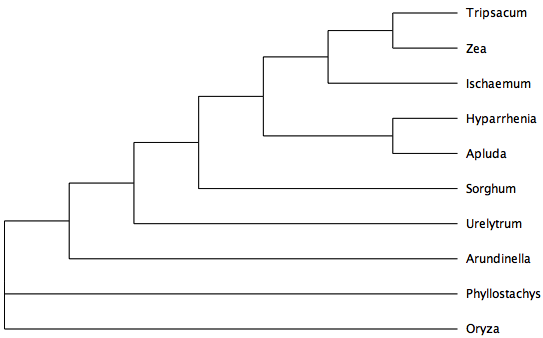
\includegraphics[width=4in]{Phylotree_centrepeat.png}
\end{center}
\caption{{\bf Cladogram of evolutionary relationships between the grasses studied.}
Topology is an approximate cladogram, reconstructed from 3 neutrally evolving loci.
A more accurate depiction of relationships is available in \cite{wu2012phylogeny}}
\label{phylotree}
\end{figure}

\subsection*{Assembly and Genomic Composition of Centromere Repeats}

% For figure citations, please use "Fig." instead of "Figure".

We used MIRA (Chevreux et al. 1999, version 4.0; job = genome,denovo,accurate, parameters = -highlyrepetitive -NW:cnfs=no -NW:mrnl=200 -HS:mnr=no) to assemble low coverage libraries.
We ran Tandem Repeat Finder \cite{benson1999tandem}  (TRF, ; parameters: 2 7 7 80 10 50 2000 -h) on all assembled contigs to select only those that contained tandem repeats.  
%Previous surveys across both plant and animal taxa show that centromere repeats are short and often the most abundant tandem repeat \cite{melters2013comparative}.  
%However, studies have shown that in certain grasses such as \emph{Zea mays} the centromere repeat is not the most abundant tandem repeat due to the presence of knobs (Not sure what to cite).
%To ensure that we were selecting the most abundant tandem repeat with no homology to known knob repeats, we identified assembled contigs with homology to known knob repeats via blastn and removed them.
%Those non-knob-like tandem repeat assemblies for each species were then used as a mapping reference for Mosaik, which stores information about multiply mapping reads (version 1.0; parameters optimized for tandem repetitive elements as in \cite{bilinski2014diversity}.
To discover the genomic composition of each tandemly repeated contig, we used Mosaik, which stores information about multiply mapping reads (version 1.0; parameters optimized for tandem repetitive elements as in \cite{bilinski2014diversity}.
Low coverage libraries were mapped against the reference and contigs were ranked by in-house scripts that quantified the number of reads aligning to each contig.
The top ranking contig was extracted, and the number of reads aligning to it was recorded from the assembly ace files.
We then blasted (-evalue 1E-1 -outfmt 7 -max\_target\_seqs 15000 -task blastn) the top ranking contig against all other TRF assemblies, removed assemblies with BLAST homology.
This process was repeated 4 times to identify the genomic composition of the 4 highest abundance tandem repeat groups.
Scripts and step by step guides are available on MY GITHUB.
%If the highest abundance contig shared homology with a known non-centromeric repeat in grasses, it was discarded.  
%From the highest abundance polymer and our TRF identifications, we extracted the single chimeric monomer produced from TRF.  
%We blasted the monomer against all other TRF assemblies, and used the monomer (narrow) and list of polymers with homology to the monomer (broad) as mapping references to identify genomic abundance of the putative centromere repeat.


\begin{figure}[h]
\begin{center}
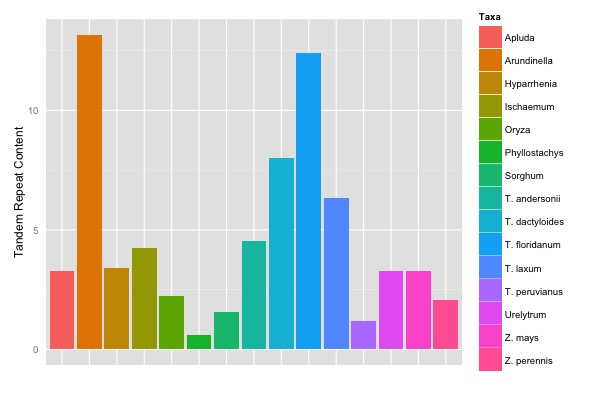
\includegraphics[width=4in]{totaltrfcontent.png}
\end{center}
\caption{{\bf Genomic composition of all tandem repeat contigs in monocot taxa.}
Values are derived from the sum of all reads mapping to any tandemly repetitive contig derived from TRF after MIRA assembly.  
Species are listed ALPHABETICALLY? probably by phylogenetic relationships shown in Fig \ref{phylotree}.}
\label{totaltrf}
\end{figure}


\subsection*{Fluorescent In-Situ Hybridization}
Sequences for FISH probes had (Udig 96\% identity; Hyp 96\% identity) as they were consensus sequences from TRF assemblies of highly similar high abundance contigs.
Rest is jiming.

%\begin{figure}[h]
%\caption{{\bf Figure Title first bold sentence Nulla mi mi, venenatis sed ipsum varius, volutpat euismod diam.}
%Figure Caption Proin rutrum vel massa non gravida. Quisque tempor sem et dignissim rutrum. A: Lorem ipsum dolor sit amet. B: Consectetur adipiscing elit.}
%\label{fig1}
%\end{figure}
%
%\begin{enumerate}
%\item{react}
%\item{diffuse free particles}
%\item{increment time by dt and go to 1}
%\end{enumerate}

% Results and Discussion can be combined.
\section*{Results}
Assembly of low coverage whole genome shotgun Illumina data produced several thousand contigs in each species from our panel.
From these, TRF was able to identify between 300 and 15,000 contigs comprised of tandem repeats in each taxa.
The number of post-TRF contigs varied between taxa based on coverage and overall genomic repetitive content.
We mapped whole genome shotgun Illumina data against all post-TRF contigs to approximate genomic composition of all tandemly repetitive sequence in our panel \ref{totaltrf}.
Mapping against all contigs enables us to capture the broad diversity of all tandem repeats.
Results show that our taxa vary greatly in their total tandem repeat content, ranging from over 13\% to under 1\%.
We see high tandem repeat content within the \emph{Tripsacum} and \emph{Arundinella} genera, though \emph{Tripsacum} taxa show large variations.
We wanted to see whether total tandem repeat content correlated with genome size.
Using the Kew C-Value database and literature (what lit do we cite?), we obtained point estimates for genome size in each of our taxa.
The correlation between total tandem repeat content and genome size was poor (r=0.05).

We further wanted to investigate the proportional contribution of the most common tandem repeat classes in each of our taxa.
To do so, we ranked the mapping abundance of all post-TRF contigs.
We used the number of reads mapping to the top ranked contig as its abundance, and removed any similar contigs from our rankings using BLAST homology (See methods for parameters).
We repeated this for the top four tandem repeats in each genome.
Results showed that most taxa had one tandem repeat class at much higher abundance than other tandem repeats.
In all taxa except for \emph{Arundinella}, only the top contig exceeded 1\% of genomic composition.
\emph{Sorghum}, \emph{Phyllostchys}, \emph{Ischaemum}, and \emph{Apluda} showed the largest difference between the top ranked contig and the second ranked contig.
In the sister genera \emph{Zea} and \emph{Tripsacum}, while the top ranked contig showed immense variation, the second ranked contig had a relatively constant abundance near half a percent.
The \emph{Arundinella} genome seems unique in that it has several high abundance different class tandem repeats.
Do I include anything about BLAST homology between contigs?

In our analysis of genomic contribution from each class of tandem repeat, we found that most genomes had one class of tandem repeat far above the rest.
Previous works have posited that this repeat is the centromeric repeat in many species \cite{melters2013comparative}.
We wanted test this hypothesis in taxa with known centromere repeats as well as in taxa with uncharacterized genomes.
For \emph{Oryza} and \emph{Sorghum}, whose centromere repeats are known, the assumption that the highest abundance tandem repeat is the centromere repeat is true.
In \emph{Zea} and \emph{Tripsacum}, where knob repeats are known to exist \cite{dennis1984knob}, the centromere repeat is not the highest abundance tandem repeat, though it is ranked within the top four.
Several other taxa (LIST) had top ranked contigs that shared homology with the \emph{Sorghum} centromere repeat, suggesting that the method is robust in these taxa as well.
However, our analyses also yielded several taxa whose top ranked contig had no homology to known centromere repeats.
We chose to test the robustness of the Melters et al (2013) assumption in these taxa with fluorescent in-situ hybridization (FISH).
In \emph{Urelytrum} and \emph{Hyparrhenia}, FISH results did not suggest that the highest ranked contig was centromeric, as probe illumination was scattered across chromosomes, not often found near central locations, or confined to only some of the chromosomes \ref{FISH}.
In \emph{Arundinella}, a taxon with a large portion of its genome comprised of tandem repeats, FISH results showed something we have yet to see though I hope it shows new knobs.
\\

\begin{figure}[h]
\begin{center}
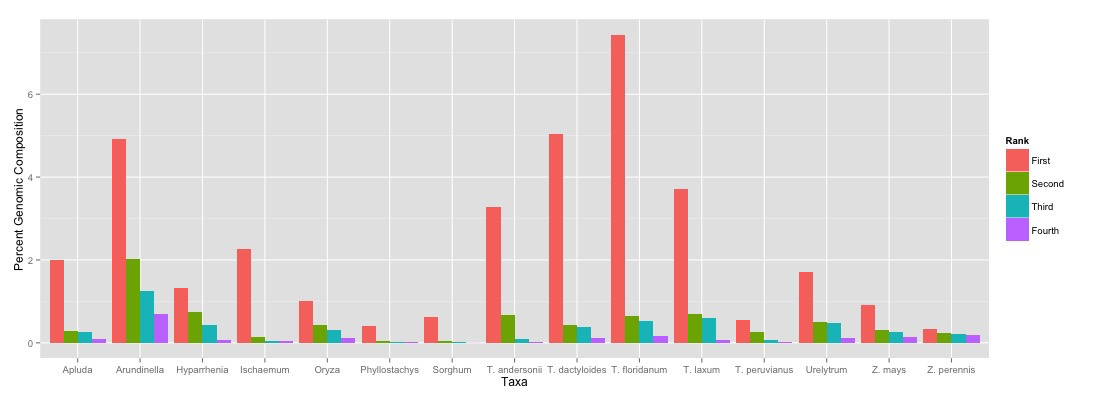
\includegraphics[width=4in]{Rankstrfcontent.png}
\end{center}
\caption{{\bf Genomic Composition of Top 4 Tandemly Repetitive Contig that do not share sequence homology.} Ain't it pretty?  Check those knobs.}
\label{ranktrf}
\end{figure}

\begin{figure}[h]
\begin{center}
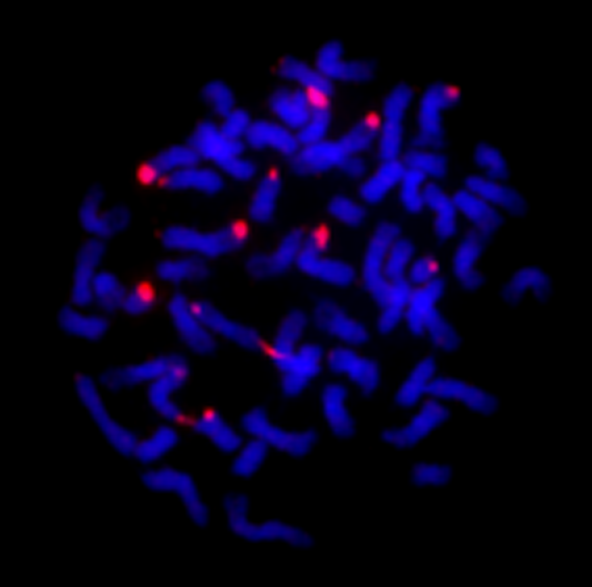
\includegraphics[width=4in]{Udig_TK271-Repeat.png}
\end{center}
\caption{{\bf .} }
\label{FISH}
\end{figure}

\begin{figure}[h]
\begin{center}
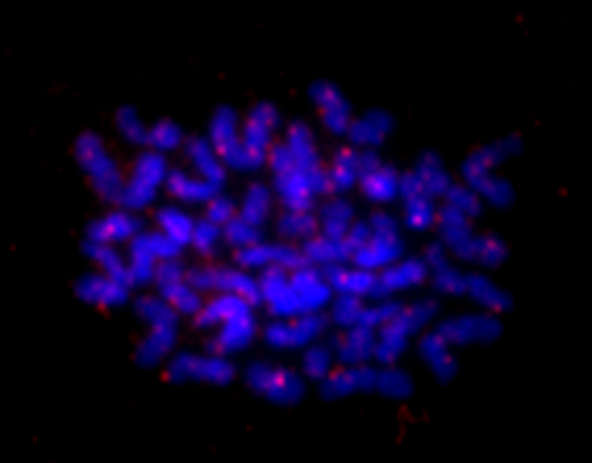
\includegraphics[width=4in]{Hypdip_TK177-Repet.png}
\end{center}
\caption{{\bf .} }
\label{FISH2}
\end{figure}


%\begin{table}[!ht]
%\begin{adjustwidth}{-2.25in}{0in} % Comment out/remove adjustwidth environment if table fits in text column.
%\caption{
%{\bf Table caption Nulla mi mi, venenatis sed ipsum varius, volutpat euismod diam.}}
%\begin{tabular}{|l|l|l|l|l|l|l|l|}
%\hline
%\multicolumn{4}{|l|}{\bf Heading1} & \multicolumn{4}{|l|}{\bf Heading2}\\ \hline
%$cell1 row1$ & cell2 row 1 & cell3 row 1 & cell4 row 1 & cell5 row 1 & cell6 row 1 & cell7 row 1 & cell8 row 1\\ \hline
%$cell1 row2$ & cell2 row 2 & cell3 row 2 & cell4 row 2 & cell5 row 2 & cell6 row 2 & cell7 row 2 & cell8 row 2\\ \hline
%$cell1 row3$ & cell2 row 3 & cell3 row 3 & cell4 row 3 & cell5 row 3 & cell6 row 3 & cell7 row 3 & cell8 row 3\\ \hline
%\end{tabular}
%\begin{flushleft} Table notes Phasellus venenatis, tortor nec vestibulum mattis, massa tortor interdum felis, nec pellentesque metus tortor nec nisl. Ut ornare mauris tellus, vel dapibus arcu suscipit sed.
%\end{flushleft}
%\label{table1}
%\end{adjustwidth}
%\end{table}



%\subsection*{\lorem\ and \ipsum\ Nunc blandit a tortor.}


% Please do not create a heading level below \subsection. For 3rd level headings, use \paragraph{}. 

\section*{Discussion}
Section 1: TRF/abundance as a way to identify de novo cent repeats (FAIL)
Section 2: Other applications: can ID novel big repeats in nonmodel systems
Section 3: Discuss genomic comp in our taxa, say we can see this method used to ID variation in genomic comp across a genus or populations, a way to start quantifying and documenting variation in repeat regions


%
%\subsection*{S2 Fig}
%\label{S2_Fig}
%{\bf Lorem Ipsum.} Maecenas convallis mauris sit amet sem ultrices gravida. Etiam eget sapien nibh. Sed ac ipsum eget enim egestas ullamcorper nec euismod ligula. Curabitur fringilla pulvinar lectus consectetur pellentesque.
%
%\subsection*{S1 Table}
%\label{S1_Table}
%{\bf Lorem Ipsum.} Maecenas convallis mauris sit amet sem ultrices gravida. Etiam eget sapien nibh. Sed ac ipsum eget enim egestas ullamcorper nec euismod ligula. Curabitur fringilla pulvinar lectus consectetur pellentesque.

\section*{Acknowledgments}
Again, shout out to the homeys.
\nolinenumbers

%\section*{References}
% Either type in your references using
% \begin{thebibliography}{}
% \bibitem{}
% Text
% \end{thebibliography}
%
% OR
%
% Compile your BiBTeX database using our plos2015.bst
% style file and paste the contents of your .bbl file
% here.
% 
\bibliography{refdenovocent.bib}



\end{document}

